% This chapter should describe what was actually produced: the programs which were written, the hardware which was built or the theory which was developed. Any design strategies that looked ahead to the testing stage should be described in order to demonstrate a professional approach was taken.

% The repository overview should be around one page in length and should describe the high-level structure of the source code found in your source code repository. It should describe whether the code was written from scratch or if it built on an existing project or tutorial.

% Contribution to the field, with genuine potential for impact outside the tripos.

% Challenging goals and substantial deliverables, all methods and tools deployed expertly.

% Original techniques or methodologies going beyond what was previously known.

% Presentation is clear and concise throughout, with creative use of figures or diagrams.

% Excellent repository overview, giving clear insight into project structure.

\label{sec:3}

\section{Agent Architectural Overview}
\label{sec:architectural-overview}

\begin{figure}[h]
    \centering
    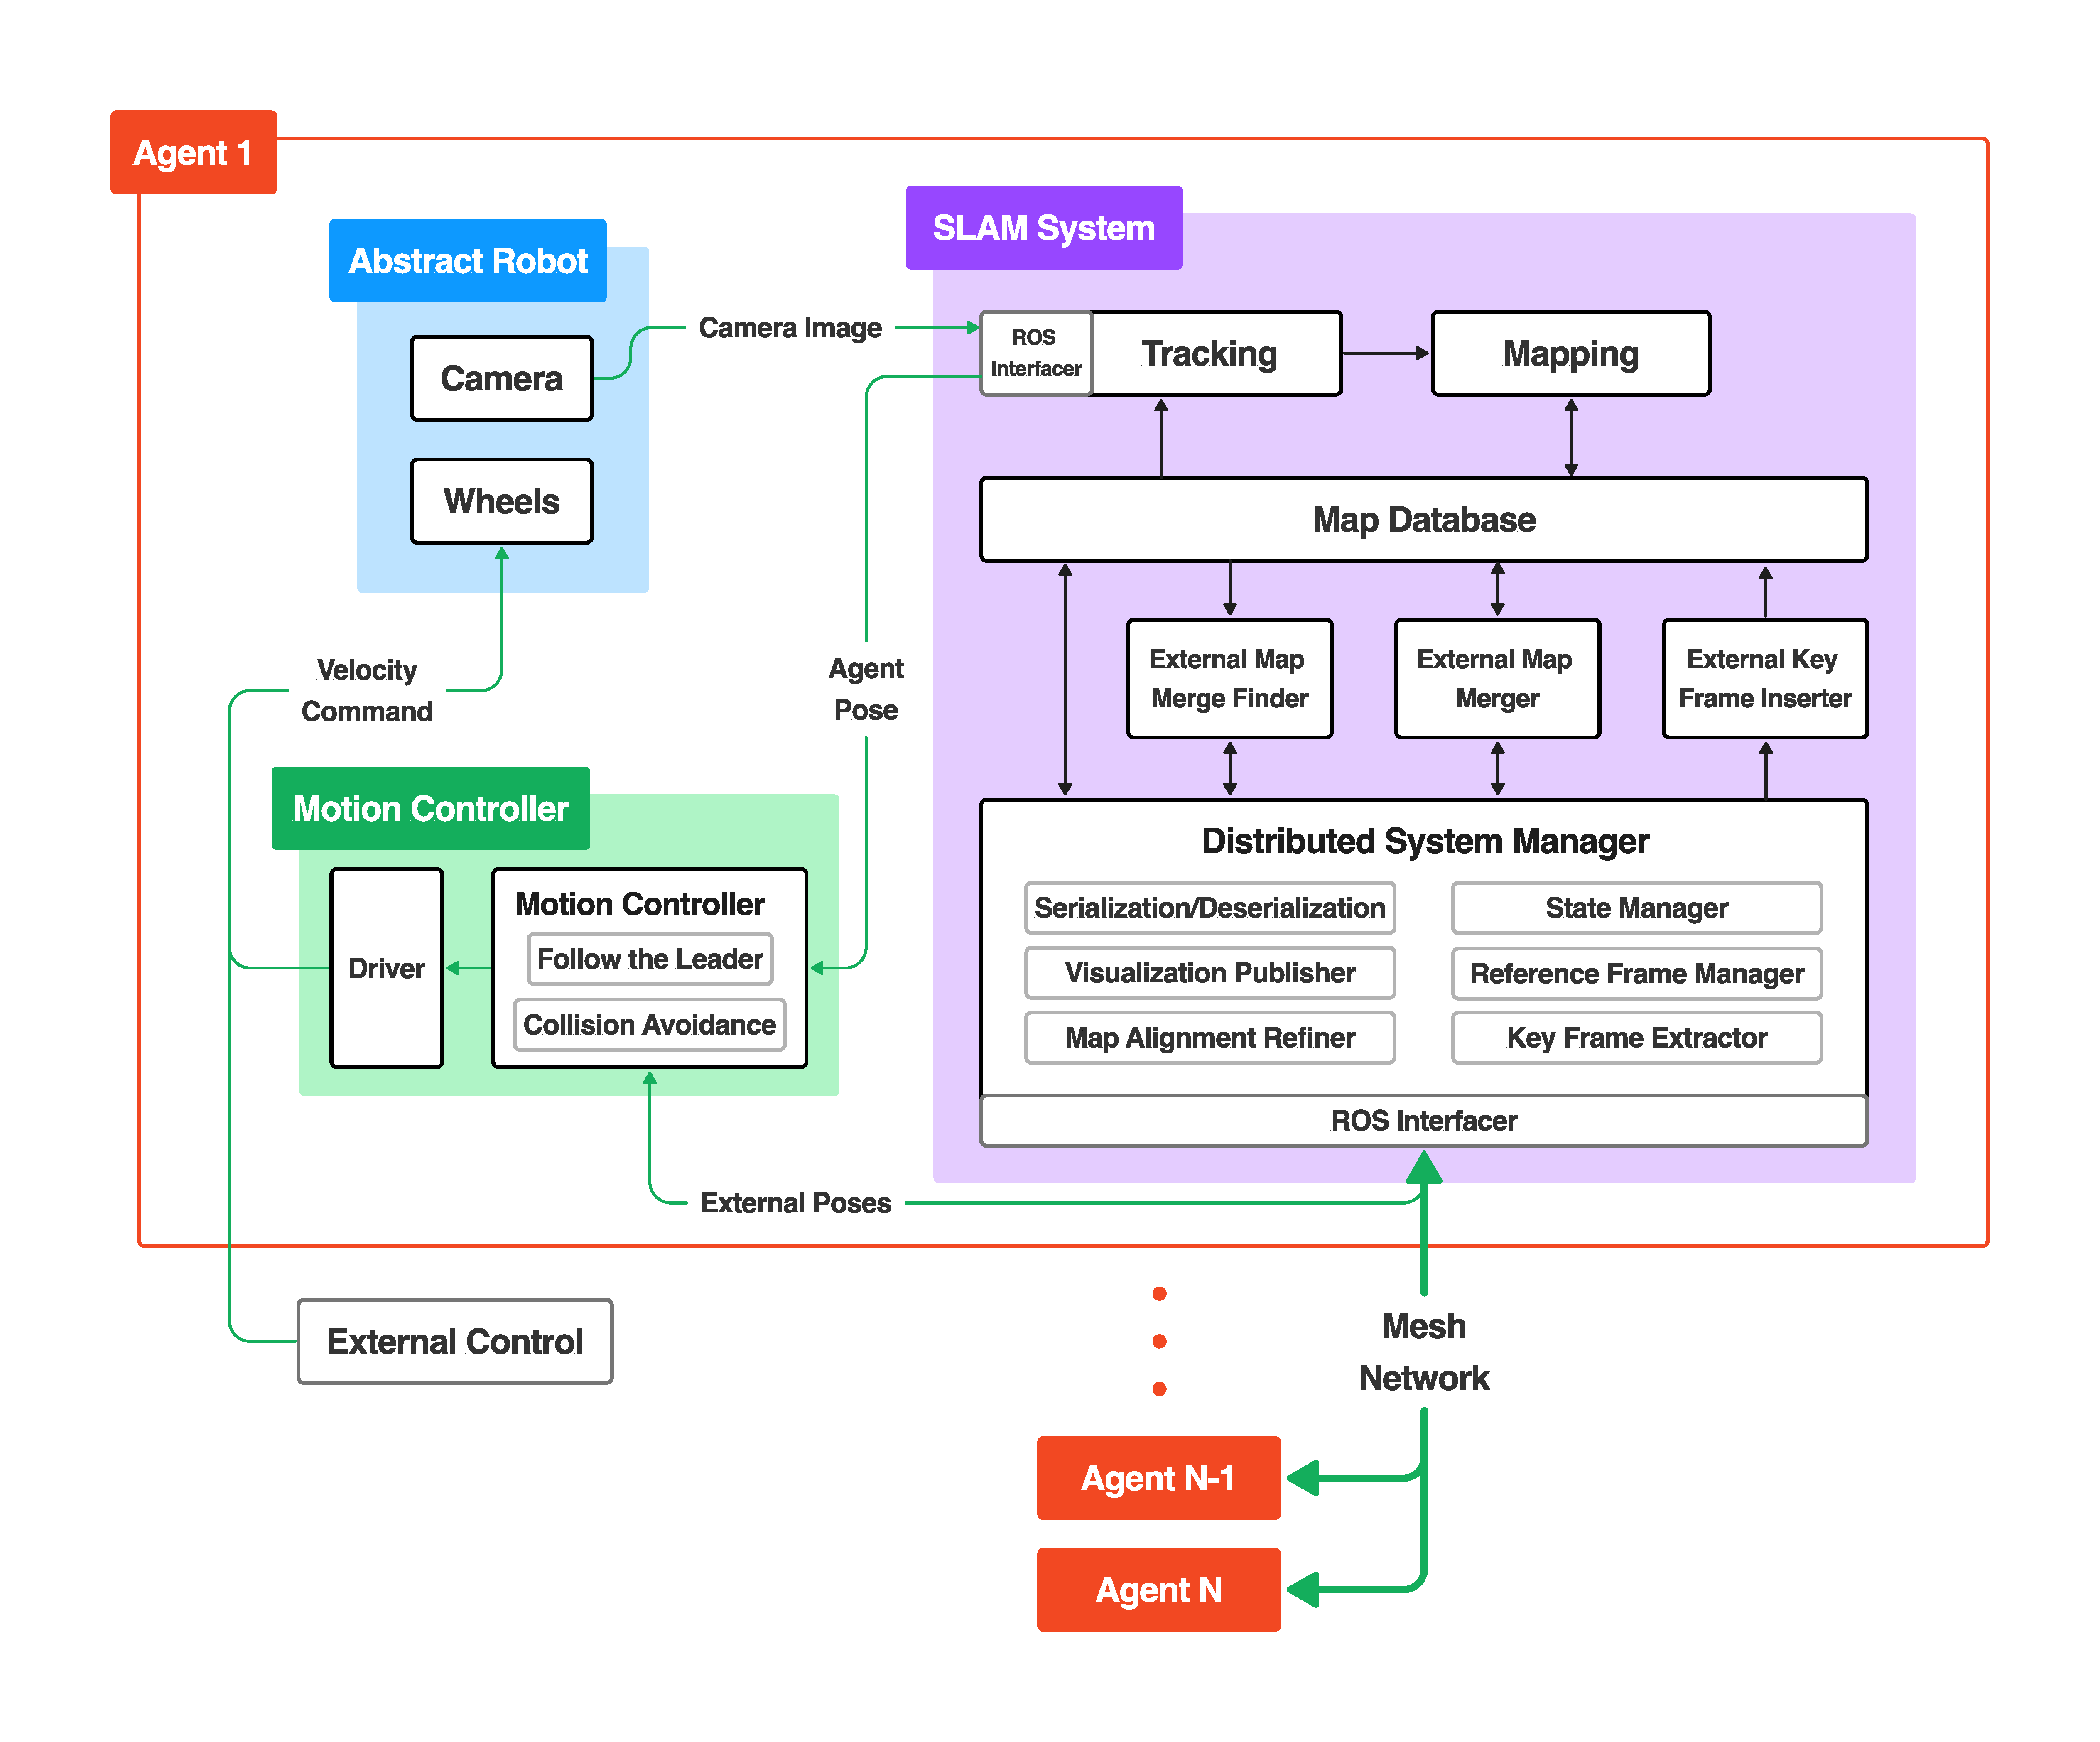
\includegraphics[trim=5cm 5cm 5cm 5cm, scale=0.2]{figures/agent_diagram.pdf}
    \caption{Agent diagram. Green arrows represent messages sent over ROS topics, while black arrows are internal communications within a node.}
    \label{fig:agent-diagram}
\end{figure}

\autoref{fig:agent-diagram} gives an architectural overview of an agent, showing how the \texttt{Abstract Robot}, \texttt{SLAM System} and \texttt{Motion Controller} ROS nodes interconnect.

From a high level, we have an \texttt{Abstract Robot} node which provides an interface to the robot's hardware, as explained in \autoref{sec:ros-2}. This sends camera images to the \texttt{SLAM System} node, which builds a map of the world in collaboration with its peers. The \texttt{Motion Controller} node receives agent pose information from both the local \texttt{SLAM System} and the external peers to perform tasks such as collision avoidance by sending velocity commands back to the \texttt{Abstract Robot} node, closing the control loop.

In the following sections, we will explore these nodes in detail.

\section{SLAM System}
\label{sec:slam-system}
The SLAM System node is the majority of this project's implementation. It processes monocular images from the camera to localize the agent while also collaboratively building up a map of the world with its peers. As discussed in \autoref{sec:starting-point}, my system is based on an existing single-agent SLAM system which performs the \texttt{Tracking} and \texttt{Mapping} tasks. While substantial modifications were made to the base single-agent system, I will generally focus on the decentralized layer I have built on top in the interest of space.

\subsection{Decentralized System Manager}
\label{sec:decentralized-system-manager}
Decentralized collaborative SLAM systems have significantly more complexity than a single-agent or even centralized collaborative system, due to the complex interactions between agents as they merge maps, lose localization, or lose connection with the network. Therefore, a robust framework must be put in place to ensure the robustness and corectness of the system, which I have implemented in the \texttt{Decentralized System Manager} component.

For the sake of simplicity, the following explanations will explore the interactions between just two agents: a \textit{local} and \textit{external} agent. However, this framework easily generalizes to a system with an arbitrary number of agents when augmented by some simple rules set out in the \textit{\nameref{sec:generalizing-to-n-2-agent-systems}} Section.

\subsubsection{State Manager}
\label{sec:state-manager}

\begin{figure}[h]
    \centering
    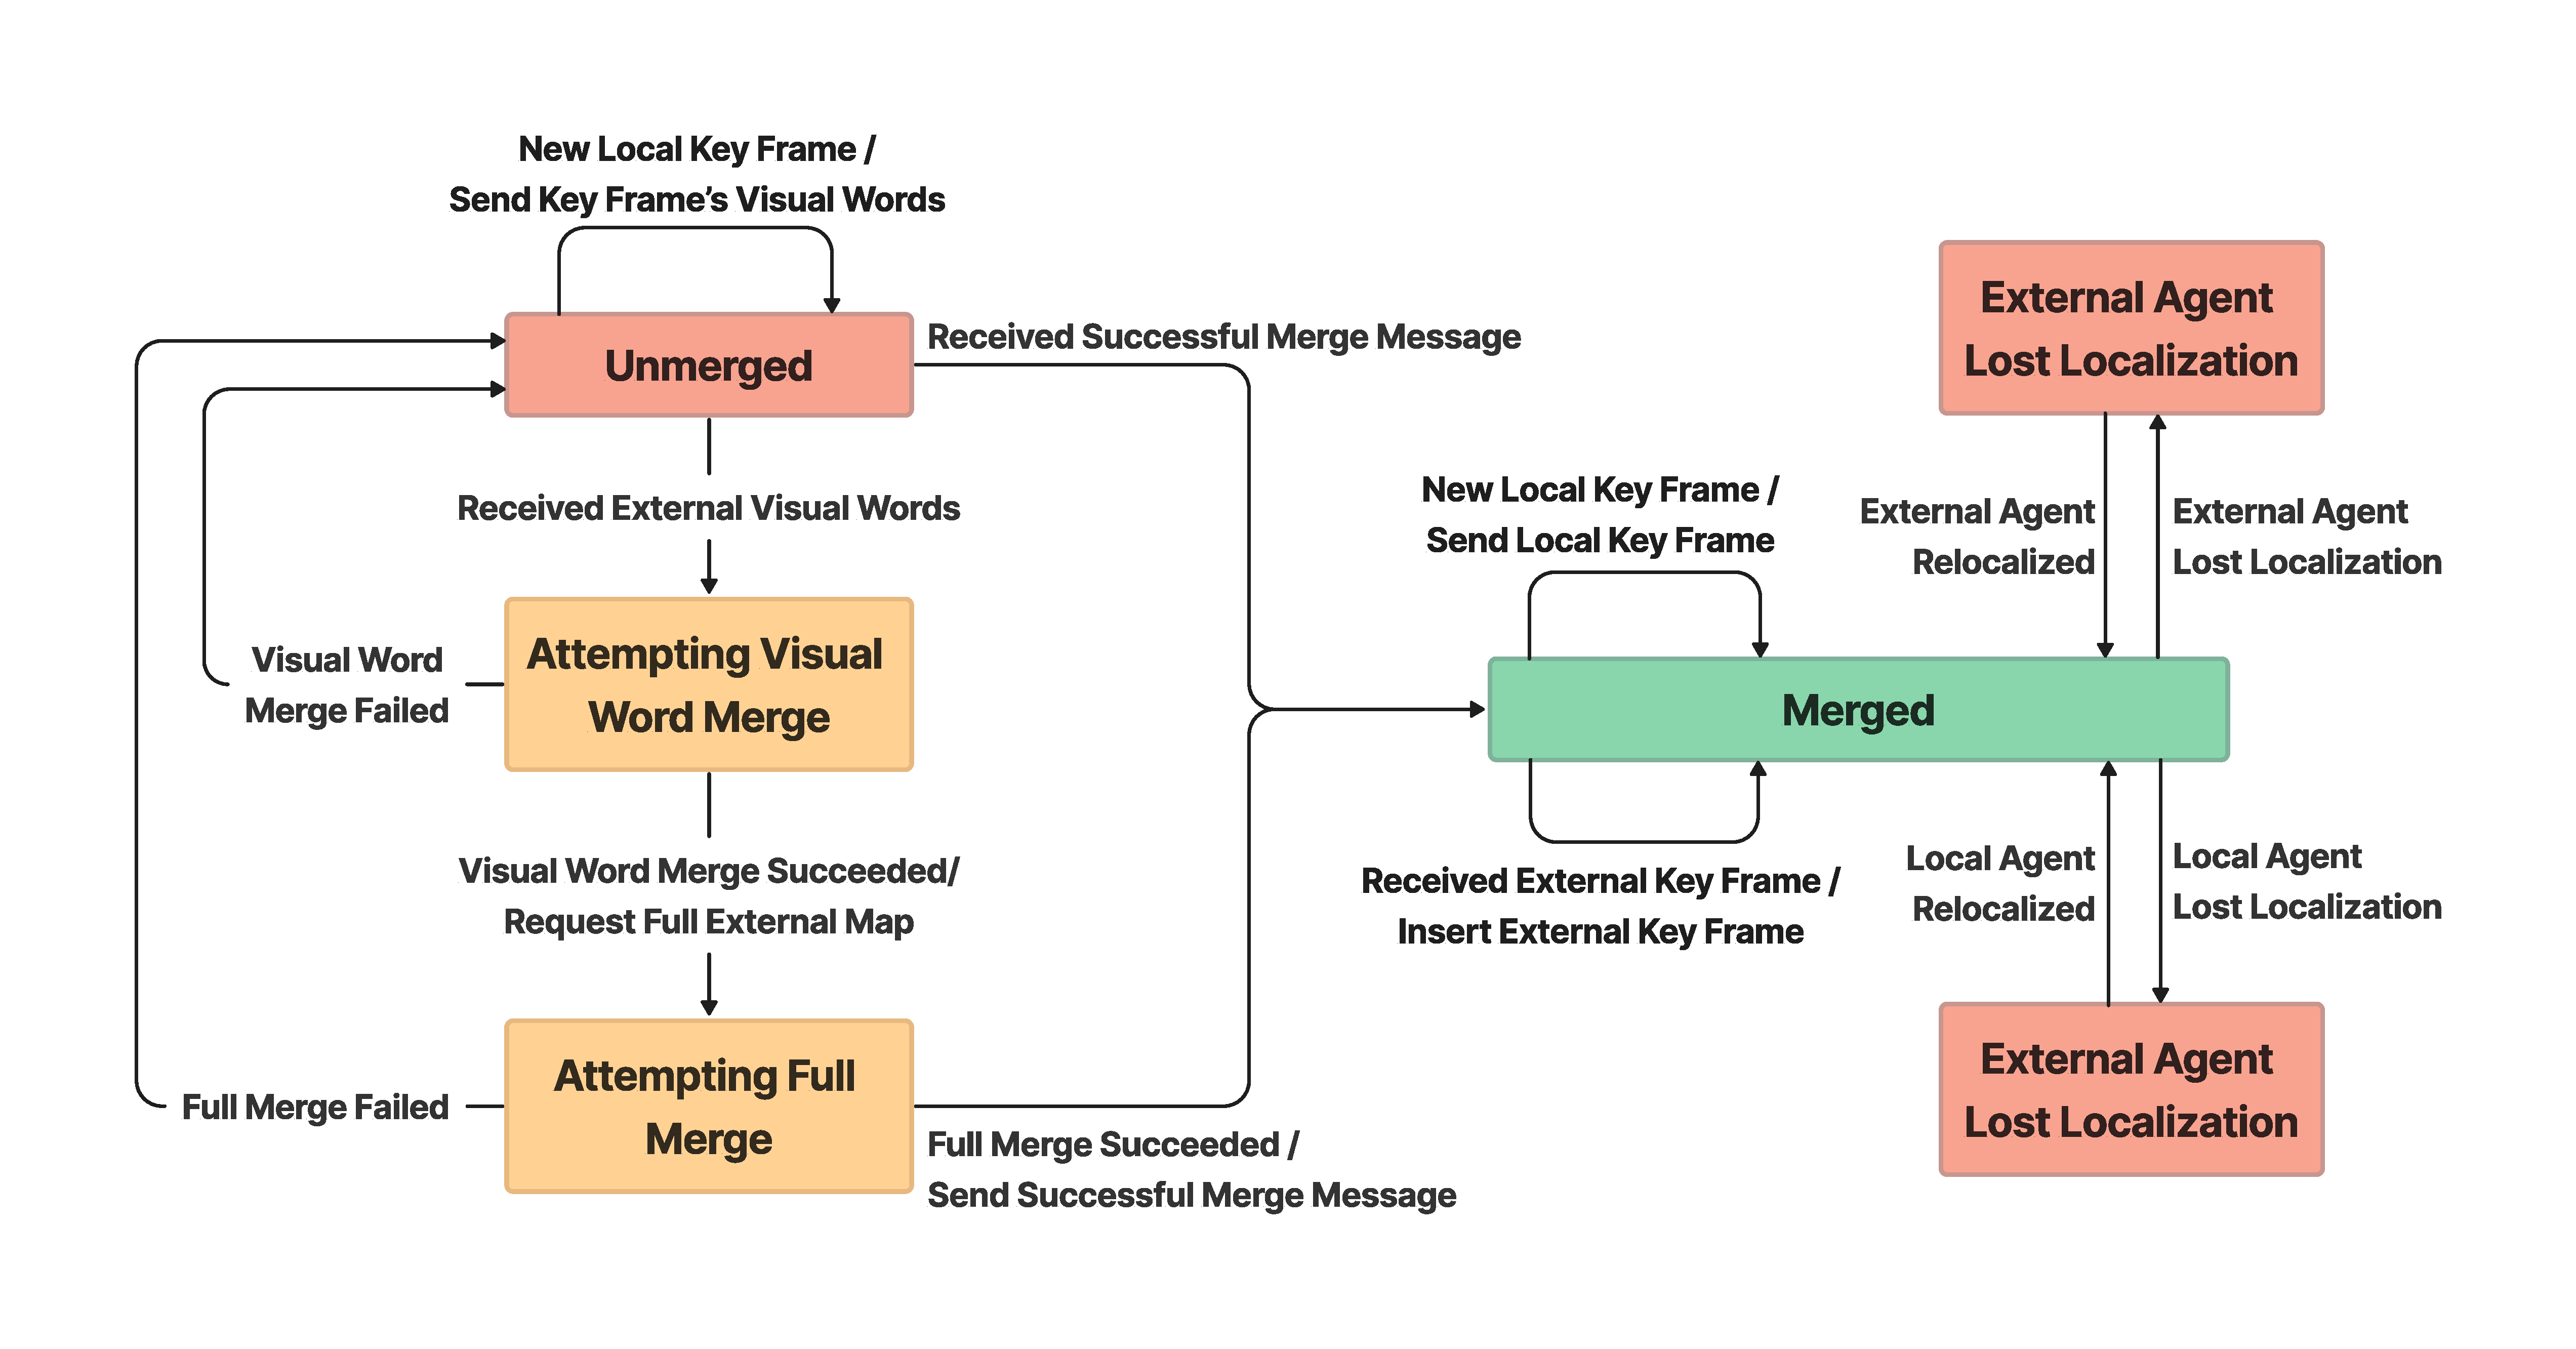
\includegraphics[trim=5cm 5cm 5cm 5cm, scale=0.2]{figures/slam_system_state_machine.pdf}
    \caption{SLAM system state machine for a single peer.}
    \label{fig:state-machine}
\end{figure}

Each agent's \texttt{Decentralized System Manager} maintains a state machine for every peer in the system, shown in \autoref{fig:state-machine}. All peers are initially in the \texttt{unmerged} state, meaning that they are in different coordinate frames and can not collaboratively build a map together. As the local agent starts to explore the same places as its peers, we are able to recognize the visual overlaps and merge their maps, bringing us to the \texttt{merged} state where the agents share the same coordinate frame and map, enabling relative positioning and collaborative map building.

\subsubsection{External Map Merge Finder}
\label{sec:external-map-merge-finder}
A naive approach to merging maps with an external agent is to constantly exchange our full maps, each time trying to identify if a map merge is possible. While simple, this approach clearly does not scale well from both a networking and computational perspective, as maps are often \>1MB in size and computing a full map merge is extremely computationally expensive.

Instead, we first identify if a map merge is even feasible by using visual words before attempting a full map merge. This eliminates superfluous map merge attempts that have no chance of succeeding because the agents' maps have no visual overlap.

As the agents generate new key frames, we calculate the \hyperref[sec:visual-bag-of-words]{visual bag of words} seen by that key frame and send them to our peers over the \texttt{/new\_key\_frame\_bows} ROS topic. These visual words are significantly smaller than sending over the complete map and enable agents to detect if there is a significant amount of visual overlap between its local map and the external agent's map. This is computed by \autoref{alg:map-merge-finder}.

This method gives a recall of almost 100\%, at the cost of potentially lower precision. This is a worthwhile tradeoff however, as it is essential to have very few false negatives so we can merge maps as soon as possible so the agents can begin collaborating and determine relative positioning. TODO: generate stats on this?

TODO: generate stats on how much this cuts down on bandwidth and computation

\begin{algorithm}
    \caption{Map merge finder using visual words. TODO: improve}
    \label{alg:map-merge-finder}
    \begin{algorithmic}[1]
        \Require{$E$: Set containing external key frame's visual words}
        \Ensure{$success$: Boolean value signaling if a merge is possible based on visual words}
        \State $(externalMergeScore,\ bestMatchKeyFrame) \gets CalculateMergeScore(E)$
        \State $I \gets ComputeVisualWords(bestMatchKeyFrame)$
        \State $(internalMergeScore,\ _) \gets CalculateMergeScore(I)$
        \State $success \gets externalMergeScore \geq internalMergeScore$
    \end{algorithmic}
\end{algorithm}

\subsubsection{External Map Merger}
\label{sec:external-map-merger}
Once a potential map merge with the external agent is identified by the \hyperref[sec:external-map-merge-finder]{external map merge finder}, we can begin a full merge attempt. We first request the full map from the external agent through the \texttt{/get\_current\_map} ROS topic. Once the map is received, we deserialize it and place it into our \textit{map database} data structure.

From this point, we need to confirm that a map merge is possible using the full map data.

TODO

Given the external key frame $k_0$ whose visual words triggered this map merge attempt, we extract a \textit{local window} $K$ of key frames connected to $k_0$ in the covisibility graph.

If the full map merge is ultimately successful, we broadcast a \texttt{/successfully\_merged} message to tell the external agent that we have successfully merged their map. The external agent will then move to the \texttt{merged} state and both agents will begin sharing key frames with each other.

It is important to note that this system requires only one agent to calculate the map merge, significantly reducing the computational overhead of map merging, especially in systems with many agents (further explained in \autoref{sec:generalizing-to-n-2-agent-systems}).

\subsubsection{Keeping Maps Merged}

\subsubsection{Local Key Frame Inserter}
\label{sec:local-key-frame-inserter}
As mentioned in the \nameref{sec:external-key-frame-inserter} section, it is essential that the local and external maps stay well connected, sharing the majority of their map points. In other words, we must

\subsubsection{External Key Frame Inserter}
\label{sec:external-key-frame-inserter}
Once the local and external agents have merged their maps and share the same coordinate frame, they can begin sharing key frames with each other.

Each agent maintains a set of sent key frames $K_{sent}$ and map points $M_{sent}$. The set of unsent key frames and map points are therefore represented as $K_{unsent} = K / K_{sent}$ and $M_{unsent} = M / M_{sent}$ respectively. Once $\#K_{unsent}$ exceeds a certain threshold, we serialize $K_{unsent}$ and $M_{unsent}$ and send them to the external agent. Finally, we add $K_{unsent}$ to $K_{sent}$ and $M_{unsent}$ to $M_{sent}$

Upon receiving the serialized key frames and map points, the external agent deserializes them and adds them to a queue to await insertion into their local copy of the shared map by the \textit{external key frame inserter}.

The external key frame inserter is run whenever we have spare cycles on the CPU, to prevent impacting the local tracking and mapping performance. The insertion process involves the following operations:

\begin{enumerate}
    \item \textbf{Pop external key frame $k_{ext}$ from front of queue}.
    \item \textbf{Relink $k_{ext}$ with covisible key frames and observed map points in the local map}. \\
          $k_{ext}$ contains references to its covisible keyframes and child map points that have already been sent or were generated by another agent. We search our local map for objects that match these references, reconnecting them.
    \item \textbf{Move $k_{ext}$ and its new external observed map points $M_{ext}$ to the local map}.
          Since the local and external agents are merged and in the same coordinate frame, we can simply move $k_{ext}$ and $M_{ext}$ to our local map without any transformations.\footnote[1]{I had previously used a \textit{key frame anchor} method, where instead of $k_{ext}$ having an absolute pose we would send its pose relative to the previous $k_{ext}$. The thought process behind this was to prevent minor misalignments between the local and external maps from preventing external key frames from properly integrating with the local map. However, experimental testing showed that this method instead caused the local and external maps to frequently diverge.}
    \item \textbf{Relink $M_{ext}$ with key frames in the local map which observe it}. \\
          $M_{ext}$ contains references to key frames which observe it which have already been sent or were generated by another agent. We search our local map for key frames that match these references, reconnecting them.
    \item \textbf{Merge $M_{ext}$ with map points in the local map}. \\
          $M_{ext}$ will already be correctly linked to observing key frames in the local map, however, due to communication latency some map points in $M_{ext}$ may be duplicates of existing map points in the local map. Therefore, we exploit spatial locality to combine duplicate map points that describe the same physical feature. A key observation was that this step is essential to ensuring the local and external keyframes stay well connected, ensuring the local and external maps do not diverge.

          TODO: add more details? idk
    \item \textbf{Perform a local bundle adjustment around $k_{ext}$}. \\
          Since we have merged map points in the previous step, we need to perform bundle adjustment to tweak the key frame and map point locations to minimize reprojection error. This helps create a more accurate map, minimizing tracking error. We also only need to perform this bundle adjustment locally, greatly reducing the computational cost.
\end{enumerate}

TODO: add diagram

\subsection{Generalizing to $N \geq 3$ Agent Systems}
\label{sec:generalizing-to-n-2-agent-systems}

\subsubsection{Map Alignment Refiner}
\label{sec:map-alignment-refiner}
As our shared map grows, the maps stored locally by the agents may "fall out of alignment". By this, we mean that the maps are slightly translated, rotated, or scaled with respect to the lead agent's map TODO: define. This is largely a side effect of our aggressive early merge strategy which may merge two agents' maps before there is significant overlap, causing the estimated map alignment (ie. transformation between the two agents' origins) to have some error.

These small alignment errors are completely acceptable when maps are small, but may cause the maps to diverge as they grow.

To remedy this problem, we continuously refine our map alignment using \nameref{sec:ransac} and the Kabsch-Umeyama point alignment algorithm. After enough changes have been made to our local map, we perform the following steps:

\begin{enumerate}
    \item \textbf{Request map point locations from the lead agent}. \\
          This is defined as the set $TaggedMP_{ext}$ where ${TaggedMP_{ext}}_i = (uuid, (x, y, z))$
    \item \textbf{Extract local map point locations}. \\
          This is defined as the set $TaggedMP_{local}$ where ${TaggedMP_{local}}_i = (uuid, (x, y, z))$
    \item \textbf{Use the Kabsch-Umeyama and RANSAC algorithms to find transform $T$ which best aligns $TaggedMP_{ext}$ to $TaggedMP_{local}$.}
          The Kabsch-Umeyama algorithm finds the SIM(3) transformation $T$ from $TaggedMP_{ext}$ to $TaggedMP_{local}$, minimizing the RMSE. However, our input data has a large number of outliers so we use RANSAC on top to find a good fit while ignoring outliers.

          The RANSAC and Kabsch-Umeyama algorithms are described in detail in \autoref{sec:ransac} and \autoref{sec:kabsch-umeyama-algorithm} respectively.
    \item \textbf{Apply transformation $T$ to our local map.}
\end{enumerate}

\subsubsection{Reference Frame Manager}
\label{sec:reference-frame-manager}

\subsubsection{Visualization Publisher}
\label{sec:visualization-publisher}

\subsubsection{Losing Localization}
\label{sec:losing-localization}

\subsection{Map Serialization and Deserialization}
\label{sec:map-serialization-and-deserialization}

\section{Motion Controller}
\label{sec:motion-controller}

\subsection{Follow The Leader}
\label{sec:follow-the-leader}

\subsection{Multi-Agent Collision Avoidance}
\label{sec:multi-agent-collision-avoidance}

\section{Custom Evaluation Suite – Multi-Agent EVO}
\label{sec:multi-agent-evo}
While there are several mature single-agent SLAM evaluation tools, I found there to be a complete lack of evaluation tools for multi-agent SLAM systems. Therefore, I have developed an open-source multi-agent SLAM evaluation tool: \textit{Multi Agent EVO}, based on the popular single agent SLAM evaluation tool \textit{EVO} \autocite{grupp2017evo}.

Besides the simple data structure and data ingestion modifications needed to allow EVO to process multi-agent SLAM data, there is some additional nuance to evaluating data from multiple agents.

Initially, all agents will be in separate reference frames until they explore an area previously seen by another agent, allowing them to merge their maps and share the same coordinate frame. We may also have cases where two independent groups of agents meet and merge maps, which requires multiple agents to simultaneously change coordinate frames. We also must note that these coordinate frames are part of the SIM(3) transformation group, which is composed of rotation, translation, and uniform scale in 3-dimensional space (scale being necessitated by the scale ambiguity of monocular visual SLAM).

Therefore, I have created a new data format to capture these changes in coordinate frames over time within our trajectory data, which Multi-Agent EVO is able to ingest. This allows us to properly compare the multi-agent SLAM trajectories to the ground truth data, giving us insights on how long it takes for agents to successfully merge maps, the accuracy of relative pose estimation, and much more.

TODO: add graph illustrating this coordinate frame stuff
TODO: perhaps list out all capabilities added

\section{Real World Implementation}
\label{sec:real-world-implementation}

\subsection{Repository Overview}
\label{sec:repository-overview}

\section{Simulation Environment}
\label{sec:simulation-environment}





